\chapter{Cross-Modal Mutual Information: CLIP and Alignment}

\section{Introduction: The Babel of Modalities}

In human cognition, information is rarely unimodal. Our understanding of the world is formed through a continuous, integrated stream of visual, auditory, and textual stimuli. When we encounter a dog, we see its shape, hear its bark, and attach the linguistic label ``dog'' to the entire sensory package. In the context of deep learning, these distinct channels of information—referred to as modalities—have historically been treated in isolation. Convolutional networks were designed to process grids of pixels, while transformers were tuned for sequences of discrete tokens. The representations learned by these architectures resided in disjoint geometric spaces; the vector representing the image of a dog bore no mathematical relationship to the vector representing the string of text ``a picture of a dog.''

The phenomenon of cross-modal alignment is the attempt to bridge this divide. By projecting different modalities into a shared latent space, models can establish a common semantic language. The breakthrough in this domain was catalyzed by Contrastive Language-Image Pretraining (CLIP), which demonstrated that vast quantities of loosely correlated image-text pairs could be leveraged to learn a highly robust, unified representation space. 

At its core, cross-modal alignment is an information-theoretic optimization problem. We are given two views of a shared underlying concept. The image and the text are both noisy, high-dimensional projections of an abstract semantic idea. Our goal is to extract the information that is common to both modalities while discarding the modality-specific noise—the exact pixel arrangement or the idiosyncratic choice of syntax. In other words, we seek representations that maximize the mutual information between the two modalities. 

However, explicitly computing the mutual information between high-dimensional continuous random variables is computationally intractable. Instead, modern alignment models rely on variational bounds. By formulating the learning objective as a contrastive task—discriminating matched image-text pairs from mismatched ones—we implicitly optimize a lower bound on the true mutual information. This chapter formalizes the cross-modal alignment process, rigorously linking the mechanics of dual-encoder architectures and the InfoNCE loss to the maximization of mutual information.

\section{The Cross-Modal InfoNCE Bound}

Let $X_1 \in \mathcal{X}_1$ represent data from the first modality (e.g., images) and $X_2 \in \mathcal{X}_2$ represent data from the second modality (e.g., text). We assume that paired observations $(x_1, x_2)$ are drawn from an unknown joint distribution $P_{X_1, X_2}$. The marginal distributions are $P_{X_1}$ and $P_{X_2}$.

We introduce two deep neural networks acting as encoders: $f_{\theta_1} : \mathcal{X}_1 \to \mathcal{Z}_1$ and $f_{\theta_2} : \mathcal{X}_2 \to \mathcal{Z}_2$, which map the input data to continuous latent representations $Z_1$ and $Z_2$. 

\begin{figure}[ht]
    \centering
    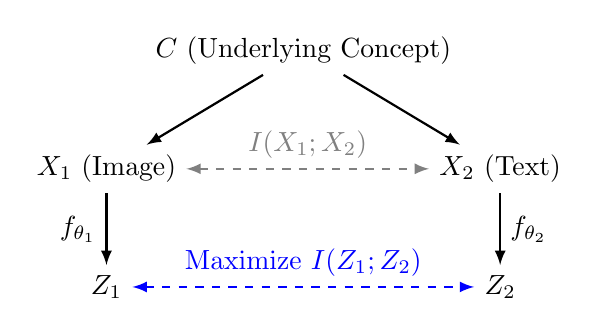
\begin{tikzpicture}[node distance=2.5cm, auto, thick, >=latex]
        % Nodes
        \node (C) at (2.5, 3) {$C$ (Underlying Concept)};
        \node (X1) at (0, 1.5) {$X_1$ (Image)};
        \node (Z1) at (0, 0) {$Z_1$};
        \node (X2) at (5, 1.5) {$X_2$ (Text)};
        \node (Z2) at (5, 0) {$Z_2$};
        
        % Arrows
        \draw[->] (C) -- (X1);
        \draw[->] (C) -- (X2);
        \draw[->] (X1) -- node[left] {$f_{\theta_1}$} (Z1);
        \draw[->] (X2) -- node[right] {$f_{\theta_2}$} (Z2);
        
        % Mutual Info Links
        \draw[<->, dashed, blue] (Z1) -- node[above] {Maximize $I(Z_1; Z_2)$} (Z2);
        \draw[<->, dashed, gray] (X1) -- node[above] {$I(X_1; X_2)$} (X2);
    \end{tikzpicture}
    \caption{The Markov structure of cross-modal alignment. The data processing inequality guarantees that $I(Z_1; Z_2) \le I(X_1; X_2)$. The objective of the encoders $f_{\theta_1}$ and $f_{\theta_2}$ is to preserve as much of the shared information derived from the true concept $C$ as possible.}
    \label{fig:clip_markov}
\end{figure}

By the Data Processing Inequality (DPI) applied to the Markov chain $Z_1 \leftarrow X_1 \leftrightarrow X_2 \rightarrow Z_2$, the mutual information between the representations is bounded by the mutual information between the raw modalities:
\begin{equation}
    I(Z_1; Z_2) \le I(X_1; X_2)
\end{equation}
Our objective is to find parameters $\theta_1, \theta_2$ that maximize $I(Z_1; Z_2)$. We approach this via contrastive estimation. Given a batch of $N$ pairs $\{(x_{1,i}, x_{2,i})\}_{i=1}^N$ drawn independent and identically distributed (i.i.d.) from $P_{X_1, X_2}$, we define a similarity scoring function (critic) $s(z_1, z_2) \in \mathbb{R}$. In CLIP, this is typically the scaled cosine similarity $s(z_1, z_2) = \frac{z_1^\top z_2}{\tau}$, where $\tau > 0$ is a temperature parameter.

The contrastive loss for predicting the correct text representation given an image representation is defined as:
\begin{equation}
    \mathcal{L}_{1 \to 2} = - \frac{1}{N} \sum_{i=1}^N \log \frac{\exp(s(z_{1,i}, z_{2,i}))}{\sum_{j=1}^N \exp(s(z_{1,i}, z_{2,j}))}
\end{equation}
This loss treats the matching text $z_{2,i}$ as the positive sample and the remaining $N-1$ texts $z_{2,j}$ in the batch as negative samples drawn from the marginal distribution $P_{Z_2}$.

\begin{theorem}[Cross-Modal InfoNCE Bound]
Let the negative samples in the denominator of $\mathcal{L}_{1 \to 2}$ be drawn i.i.d. from the marginal distribution $P_{Z_2}$. For any scoring function $s(z_1, z_2)$, the expected contrastive loss bounds the mutual information between the latent representations:
\begin{equation}
    I(Z_1; Z_2) \ge \log N - \mathbb{E}\left[\mathcal{L}_{1 \to 2}\right]
\end{equation}
\end{theorem}

\begin{proof}
Consider the optimal choice for the critic function $s^*(z_1, z_2)$. In a classification task where one seeks to identify the positive pair among $N$ choices (one positive drawn from the joint $P_{Z_1, Z_2}$ and $N-1$ negatives drawn from the product of marginals $P_{Z_1}P_{Z_2}$), the optimal classifier models the posterior probability of a sample coming from the joint distribution. 

By Bayes' theorem, the probability that the $i$-th sample is the positive pair, given the set of candidate pairs $S_i = \{ (z_{1,i}, z_{2,j}) \}_{j=1}^N$, is exactly:
\begin{equation}
    p(C=i | S_i) = \frac{\frac{p(z_{1,i}, z_{2,i})}{p(z_{1,i})p(z_{2,i})}}{\sum_{j=1}^N \frac{p(z_{1,i}, z_{2,j})}{p(z_{1,i})p(z_{2,j})}}
\end{equation}
This implies the optimal score function is proportional to the log density ratio: $s^*(z_1, z_2) = \log \frac{p(z_1, z_2)}{p(z_1)p(z_2)} + \text{const}$.

Substituting the optimal critic into the expected loss:
\begin{align*}
    \mathbb{E}\left[\mathcal{L}_{1 \to 2}\right] &= \mathbb{E}_{S} \left[ - \log \frac{\frac{p(z_1, z_2)}{p(z_1)p(z_2)}}{\frac{p(z_1, z_2)}{p(z_1)p(z_2)} + \sum_{j \neq i} \frac{p(z_1, z_{2,j})}{p(z_1)p(z_{2,j})}} \right] \\
    &= \mathbb{E}_{S} \left[ \log \left( 1 + \frac{p(z_1)p(z_2)}{p(z_1, z_2)} \sum_{j \neq i} \frac{p(z_1, z_{2,j})}{p(z_1)p(z_{2,j})} \right) \right]
\end{align*}
By Jensen's inequality applied to the concave $\log$ function, we can move the expectation inside for the terms involving the negative samples:
\begin{align*}
    \mathbb{E}\left[\mathcal{L}_{1 \to 2}\right] &\ge \mathbb{E}_{(Z_1,Z_2)\sim P_{Z_1, Z_2}} \left[ \log \left( 1 + \frac{p(z_1)p(z_2)}{p(z_1, z_2)} (N-1) \mathbb{E}_{z_{2}' \sim P_{Z_2}} \left[ \frac{p(z_1, z_{2}')}{p(z_1)p(z_{2}')} \right] \right) \right]
\end{align*}
Since $\mathbb{E}_{z_{2}' \sim P_{Z_2}} \left[ \frac{p(z_1, z_{2}')}{p(z_1)p(z_{2}')} \right] = \int p(z_{2}') \frac{p(z_1|z_{2}')}{p(z_1)} dz_{2}' = \frac{p(z_1)}{p(z_1)} = 1$, we have:
\begin{align*}
    \mathbb{E}\left[\mathcal{L}_{1 \to 2}\right] &\ge \mathbb{E}_{P_{Z_1, Z_2}} \left[ \log \left( 1 + \frac{p(z_1)p(z_2)}{p(z_1, z_2)} (N-1) \right) \right] \\
    &\approx \mathbb{E}_{P_{Z_1, Z_2}} \left[ \log \left( N \frac{p(z_1)p(z_2)}{p(z_1, z_2)} \right) \right] \quad \text{for large } N \\
    &= \log N - \mathbb{E}_{P_{Z_1, Z_2}} \left[ \log \frac{p(z_1, z_2)}{p(z_1)p(z_2)} \right] \\
    &= \log N - I(Z_1; Z_2)
\end{align*}
Rearranging terms yields $I(Z_1; Z_2) \ge \log N - \mathbb{E}\left[\mathcal{L}_{1 \to 2}\right]$.
\end{proof}

\section{Symmetry and Dual-Encoder Dynamics}

The bound derived above considers the prediction of text from images. By symmetry, the task of predicting an image from text yields the conjugate loss:
\begin{equation}
    \mathcal{L}_{2 \to 1} = - \frac{1}{N} \sum_{i=1}^N \log \frac{\exp(s(z_{1,i}, z_{2,i}))}{\sum_{k=1}^N \exp(s(z_{1,k}, z_{2,i}))}
\end{equation}
While $\mathcal{L}_{1 \to 2}$ normalizes over the text embeddings in the batch, $\mathcal{L}_{2 \to 1}$ normalizes over the image embeddings. In practice, the distributions of image embeddings and text embeddings can have different geometries and varying degrees of mode collapse. To ensure a balanced optimization that penalizes "hub" vectors in both modality spaces, the complete CLIP objective averages both directions:
\begin{equation}
    \mathcal{L}_{\text{CLIP}} = \frac{1}{2} \left( \mathcal{L}_{1 \to 2} + \mathcal{L}_{2 \to 1} \right)
\end{equation}

\begin{figure}[ht]
    \centering
    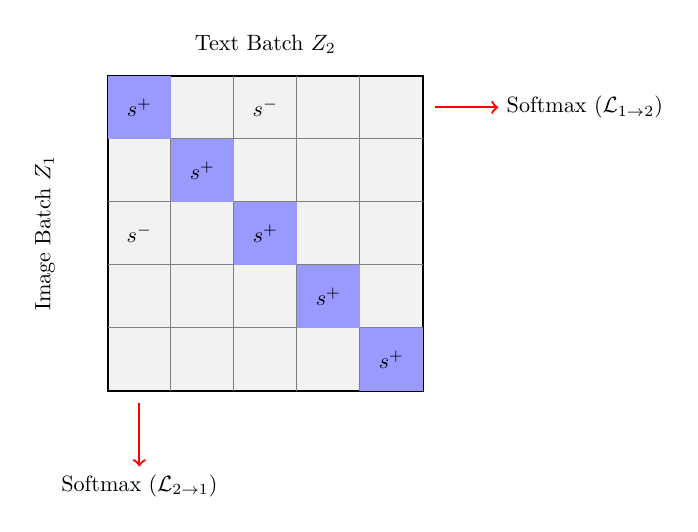
\begin{tikzpicture}[scale=0.8, transform shape]
        % Draw matrix
        \draw[thick, fill=gray!10] (0,0) rectangle (5,5);
        \foreach \i in {1,2,3,4} {
            \draw[gray] (0,\i) -- (5,\i);
            \draw[gray] (\i,0) -- (\i,5);
        }
        % Diagonal
        \foreach \i in {0,1,2,3,4} {
            \fill[blue!40] (\i, 4-\i) rectangle (\i+1, 5-\i);
            \node at (\i+0.5, 4.5-\i) {$s^+$};
        }
        
        % Off-diagonals (example)
        \node at (2.5, 4.5) {$s^-$};
        \node at (0.5, 2.5) {$s^-$};

        % Text nodes
        \node[rotate=90] at (-1, 2.5) {Image Batch $Z_1$};
        \node at (2.5, 5.5) {Text Batch $Z_2$};
        
        % Braces and labels
        \draw[thick, ->, red] (5.2, 4.5) -- (6.2, 4.5) node[right, black] {Softmax ($\mathcal{L}_{1 \to 2}$)};
        \draw[thick, ->, red] (0.5, -0.2) -- (0.5, -1.2) node[below, black] {Softmax ($\mathcal{L}_{2 \to 1}$)};
        
    \end{tikzpicture}
    \caption{The pairwise similarity matrix computed during a forward pass of CLIP. The objective maximizes the similarities on the diagonal (positive pairs $s^+$) while minimizing the off-diagonal elements (negative pairs $s^-$). The symmetric loss computes softmax cross-entropies across both rows and columns.}
    \label{fig:clip_matrix}
\end{figure}

This dual maximization restricts the encoders from ignoring the statistical structures of either domain. The true mutual information is symmetric, $I(Z_1; Z_2) = I(Z_2; Z_1)$, and both losses operate as strict lower bounds on the same underlying quantity. By optimizing their average, the training dynamics become more stable, mitigating gradients that might aggressively push one modality into a degenerate state.

\section{A Numerical Example: The Batch Size Bottleneck}

To build intuition for the bound $I(Z_1; Z_2) \ge \log N - \mathcal{L}$, consider a stylized numerical example. Suppose the shared semantic concept $C$ is a standard normal scalar $C \sim \mathcal{N}(0, 1)$. The modalities are noisy projections of this concept:
\begin{align*}
    X_1 &= C + \epsilon_1 \\
    X_2 &= C + \epsilon_2
\end{align*}
where $\epsilon_1, \epsilon_2 \sim \mathcal{N}(0, \sigma^2)$ are independent Gaussian noise. 
The joint distribution of $(X_1, X_2)$ is bivariate Gaussian with mean zero and covariance matrix:
\begin{equation}
    \Sigma = \begin{pmatrix} 1 + \sigma^2 & 1 \\ 1 & 1 + \sigma^2 \end{pmatrix}
\end{equation}
The true mutual information can be calculated precisely using differential entropy:
\begin{align*}
    I(X_1; X_2) &= h(X_1) + h(X_2) - h(X_1, X_2) \\
    &= \frac{1}{2} \log (2\pi e (1+\sigma^2)) + \frac{1}{2} \log (2\pi e (1+\sigma^2)) - \frac{1}{2} \log ( (2\pi e)^2 |\Sigma| ) \\
    &= \frac{1}{2} \log \left( \frac{(1+\sigma^2)^2}{(1+\sigma^2)^2 - 1} \right) = \frac{1}{2} \log \left( 1 + \frac{1}{2\sigma^2 + \sigma^4} \right)
\end{align*}

Observe what happens as the noise $\sigma \to 0$: the mutual information $I(X_1; X_2)$ diverges to infinity, meaning the variables perfectly determine each other. However, our InfoNCE bound is rigorously capped:
\begin{equation}
    \log N - \mathcal{L}_{1 \to 2} \le \log N
\end{equation}
Because the cross-entropy loss $\mathcal{L}_{1 \to 2}$ is non-negative, the tightest our bound can ever become is $\log N$. 
If we use a batch size of $N=256$, the maximum mutual information the loss function can ever ``see'' is $\log(256) \approx 5.54$ nats. If the true mutual information between an image and its caption requires $10$ nats to capture all granular semantic details (colors, object counts, backgrounds), a batch size of $256$ is mathematically incapable of providing gradients that encourage the encoders to capture those finer details once $5.54$ nats of information are already shared. The critic saturates.

This simple numerical artifact explains a core engineering reality of modern cross-modal models: they require exorbitant batch sizes. CLIP was trained with a batch size of $N=32,768$ (yielding a maximum bound of $\approx 10.4$ nats) specifically to raise the ceiling on the mutual information estimator, forcing the model to align on subtle, intricate semantics rather than just obvious, surface-level features.

\begin{horizon}
The mathematical necessity of massive batch sizes in contrastive learning highlights a fundamental vulnerability: the strict reliance on negative samples to formulate a partition function. It is conjectured that future multimodal architectures will entirely abandon InfoNCE in favor of non-contrastive redundancy-reduction criteria, such as those seen in Barlow Twins, scaling them across continuous multimodal domains.

A significant open question remains regarding the nature of the ``shared subspace'' $I(Z_1; Z_2)$. While current models successfully map nouns to objects, it is suspected that this intersection captures only a superficial projection of semantics. Does the geometry of the text latent space truly warp to adopt the spatial symmetries of the image space? Or does the model simply hash co-occurring patterns into arbitrary but matching clusters? 

Future work might show that simply maximizing $I(Z_1; Z_2)$ is insufficient for true multimodal reasoning. We may require structural constraints—perhaps mapping text not to points, but to functional transformations that operate on the image manifold—to graduate from mere alignment to compositional multimodal understanding.
\end{horizon}

\section{Summary}
In this chapter, we explored the information-theoretic foundations of cross-modal alignment, focusing on the CLIP architecture. We demonstrated that aligning image and text vectors via a contrastive loss is equivalent to maximizing a variational lower bound on their mutual information. Through the InfoNCE derivation, we established that the bound is strictly capped by $\log N$, dictating the necessity of massive batch sizes in practice. Furthermore, the symmetric loss formulation ensures stable representation learning by balancing the negative sampling over both marginal distributions.

\section{Exercises}
\begin{enumerate}
    \item \textbf{Temperature Scaling:} In CLIP, the similarity function is scaled by a learned temperature $\tau$, such that $s(z_1, z_2) = \frac{z_1^\top z_2}{\tau}$. Prove that if the embeddings $Z_1, Z_2$ are unconstrained (i.e., not normalized to the unit hypersphere), the temperature parameter $\tau$ is mathematically redundant and can be absorbed into the weights of the encoders. 
    \item \textbf{Biased Negatives:} The derivation of the InfoNCE bound assumes that negative samples are drawn i.i.d. from the true marginal distribution $P_{Z_2}$. Suppose instead that the batch is constructed using ``hard negatives''—samples drawn from a biased distribution $Q_{Z_2}$ that overweights items similar to $Z_1$. Derive the modified lower bound on $I(Z_1; Z_2)$ under this sampling strategy. How does the penalty term relate to the Kullback-Leibler divergence $D_{\text{KL}}(Q_{Z_2} \parallel P_{Z_2})$?
    \item \textbf{Multimodal Saturation:} Extend the bivariate Gaussian example. Suppose there are three modalities $X_1, X_2, X_3$ all generated from $C \sim \mathcal{N}(0,1)$ with independent noise variance $\sigma^2$. If we optimize pairwise CLIP losses between all three pairs, what is the theoretical maximum mutual information $I(Z_1; Z_2; Z_3)$ that can be bounded, assuming a batch size of $N$ across all modalities?
\end{enumerate}

% TODO-CITE: Ensure all named results are cited.
